
\section{ Распределения }
На рисунках 1-6 представлены графики для различных хэш функций:

\noindent\begin{minipage}[h!]{0.45\linewidth}
    \begin{center}
        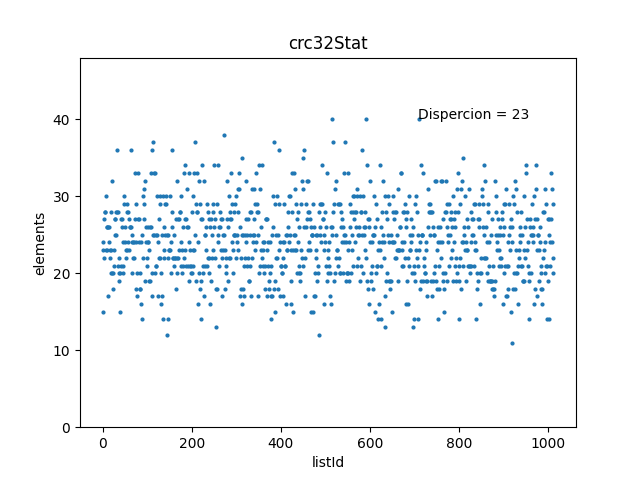
\includegraphics[width = 1\linewidth]{picks/crc32Stat.png} \\
        \textit{Рис. 1. }
    \end{center} 
\end{minipage}
\begin{minipage}[h!]{0.45\linewidth}
    \begin{center}
        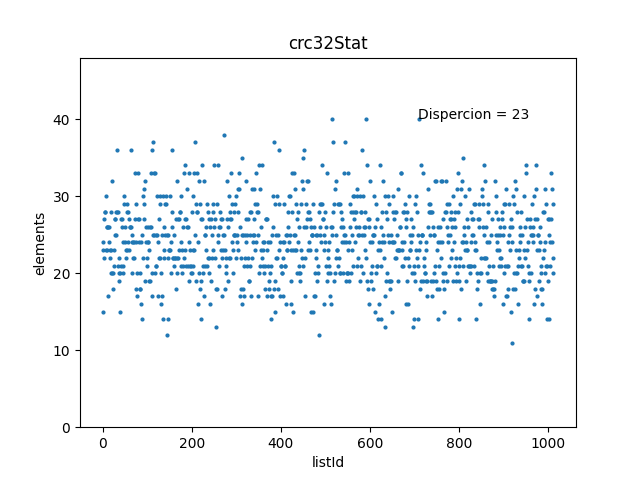
\includegraphics[width = 1\linewidth]{picks/crc32Stat.png} \\
        \textit{Рис. 2. }
    \end{center} 
\end{minipage}

\noindent\begin{minipage}[h!]{0.45\linewidth}
    \begin{center}
        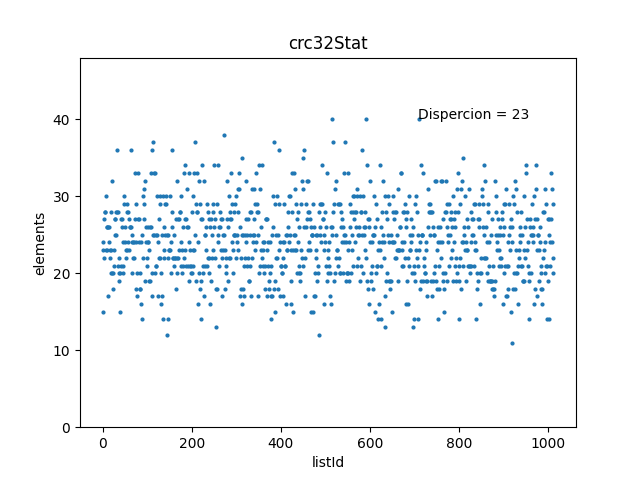
\includegraphics[width = 1\linewidth]{picks/crc32Stat.png} \\
        \textit{Рис. 3. }
    \end{center} 
\end{minipage}
\begin{minipage}[h!]{0.45\linewidth}
    \begin{center}
        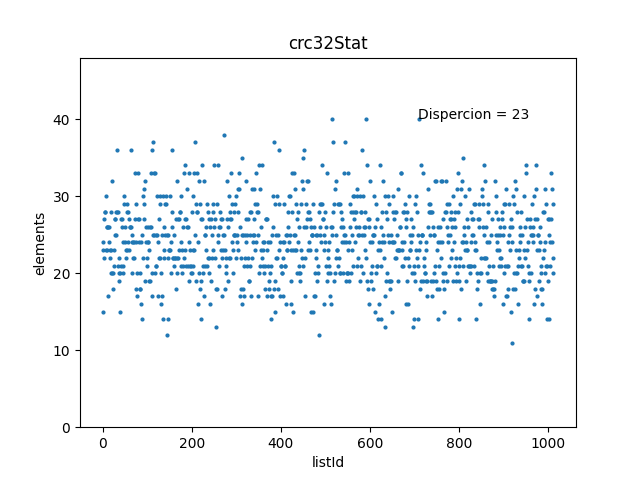
\includegraphics[width = 1\linewidth]{picks/crc32Stat.png} \\
        \textit{Рис. 1. }
    \end{center} 
\end{minipage}

\noindent\begin{minipage}[h!]{0.45\linewidth}
    \begin{center}
        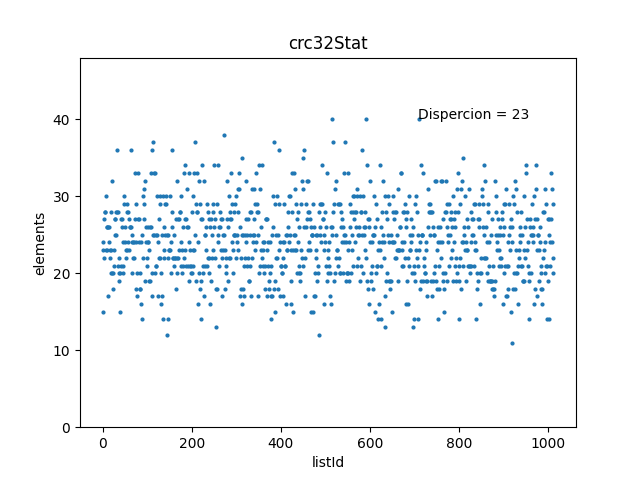
\includegraphics[width = 1\linewidth]{picks/crc32Stat.png} \\
        \textit{Рис. 4. }
    \end{center} 
\end{minipage}
\begin{minipage}[h!]{0.45\linewidth}
    \begin{center}
        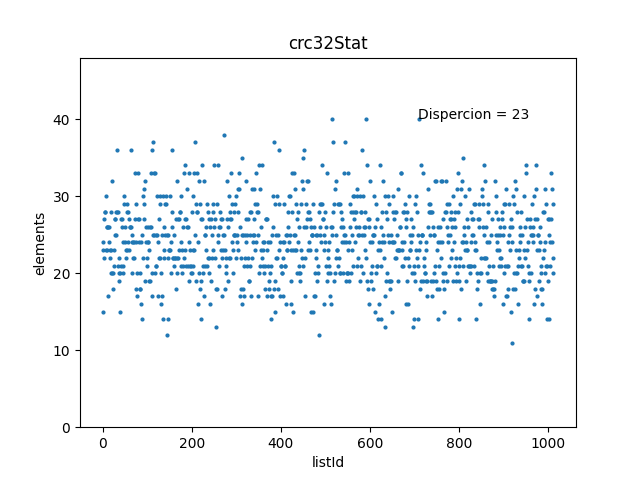
\includegraphics[width = 1\linewidth]{picks/crc32Stat.png} \\
        \textit{Рис. 5. }
    \end{center} 
\end{minipage}

\newpage

\section{ Вывод }

Видно, что лучше всего себя показывает crc32. Его я и буду использовать для следующей лабараторной работы.